\section{Fouls and Misconduct}\label{sec:fouls-and-misconduct}

Fouls and misconduct are penalised as follows:

\subsection{Direct Free Kick}\label{subsec:fouls-and-misconduct-direct-free-kick}
A direct free kick is awarded to the opposing team if a robot commits any of the following three offences:
\begin{itemize}
\item makes substantial contact with an opponent
\item holds an opponent
\item holds the ball deliberately (except for the goalkeeper within his own defence area)
\end{itemize}

\subsection{Penalty Kick}
A penalty kick is awarded if any of the offences listed in \autoref{subsec:fouls-and-misconduct-direct-free-kick} is committed by a robot inside his own defence area, irrespective of the position of the ball, provided it is in play.

A penalty kick is also awarded to the opposing team if, while the ball is in play, a defender other than the goalkeeper touches the ball while positioned entirely within the defense area.

\subsection{Indirect Free Kicks}\label{subsec:fouls-and-misconduct-indirect-free-kicks}
An indirect free kick is awarded to the opposing team if a goalkeeper, inside his own defence area, commits any of the following offences:
\begin{itemize}
\item takes more than fifteen seconds while holding the ball before releasing it from his possession
\item holds the ball again after it has been released from his possession and has not touched any other robot
\end{itemize}

An indirect free kick is also awarded to the opposing team if a robot:
\begin{itemize}
\item contacts the opponent goalkeeper where the point of contact is in the defence area
\item dribbles the ball \removed{over a distance greater than 500\,mm}
\added{over 1000 mm, measured linearly from the ball location where the
dribbling started}
\item touches the ball such that the top of the ball travels more than 150\,mm from the ground, and the ball subsequently enters their opponent's goal, without having either touched a teammate (while below 150\,mm) or remained in contact with the ground (stopped bouncing).
\item kicks the ball such that it exceeds 8\,m/s in speed
\item tips over, breaks or drops parts on the field in a way that gives its team unfair advantage
\removed{\item touches the ball such that the top of the ball travels more than
150\,mm from the ground, and the ball subsequently crosses the midline, without
having either touched another robot or the ground}
\item \added{touches the ball such that the ball, without touching any other
  robot, subsequently crosses the  midline and then the opponent's goal line
  without entering the opponent's goal}
\added{\item touches the ball while in play, while being located partially or
entirely within its opponent's defense area}
\item commits any other offence, not previously mentioned in \autoref{sec:fouls-and-misconduct}, for which play is stopped to caution or dismiss a robot
\end{itemize}

\subsection{Disciplinary Sanctions}\label{subsec:fouls-and-misconduct-disciplinary-sanctions}
\subsubsection{Cautionable Offences}
A team is cautioned and shown the yellow card if a robot on that team commits any of the following offences:
\begin{enumerate}
\item is guilty of unsporting behaviour
\item is guilty of serious and violent contact
\item persistently infringes the Laws of the Game
\item delays the restart of play
\item fails to respect the required distance when play is restarted with a goal kick, corner kick or free kick
\item modifies or damages the field or ball
\item deliberately enters or travels within the referee walking area
\item is a robot other than the goalkeeper, and touches the ball while in play, while being located partially but not entirely within \removed{the} \added{its own} defense area
\item travels faster than \removed{1\,m/s} \added{1.5\,m/s} while the ball is
out of play, no restart of play has been called, and the game is in neither a
time-out, half-time, nor similar break in gameplay such as the interval before
extra time or a penalty shootout \removed{(for games on the double-size field,
the speed limit is increased to 1.5\,m/s)}
\end{enumerate}

Upon receipt of a yellow card, the number of robots allowed on the field for the penalised team decreases by one.
If, after this decrease, the team has more robots than permitted on the field, a robot must immediately be removed from the field before play resumes.

After two minutes of play (as measured by the assistant referee using the official game time), the yellow card expires and the number of robots allowed increases by one.
The team is then permitted to place an additional robot on the field; as with all robot handling activities, this must be done with the referee's permission at a stoppage in play (as per \autoref{subsubsec:number-of-robots-interchange}).

The specific choice of robot to remove from and return to the field is made by the penalised team, and interchanges are permitted as usual under \autoref{subsubsec:number-of-robots-interchange} while one or more yellow cards are in force as long as the number of robots permitted on the field is not exceeded.

\subsubsection{Sending-Off Offences}
A team is shown a red card if one of the robots or the team is guilty of severe unsporting behaviour.

Each red card decreases the number of robots allowed on the field for the penalised team for the remainder of the game.
As with yellow cards, if a robot must be removed from the field, this is done immediately before play resumes.
Furthermore, as with yellow cards, receipt of a red card does not affect a team's ability to interchange robots under \autoref{subsubsec:number-of-robots-interchange} as long as the number of robots permitted on the field is not exceeded.

\subsection*{Decisions of the Small Size League Technical Committee}
\begin{enumerate}
\item
Substantial contact is contact sufficient to dislodge the robot from its current orientation, position, or motion in the case where it is moving.
When both robots are moving at similar speeds, and the cause of contact is not obvious, the referee will allow play to continue.
This law is designed to protect robots which are slow moving or stationary at the time of the contact, and as such should be detected by obstacle avoidance systems.

\item
Cautions for serious and violent contact are a way to discourage teams from ignoring the spirit of the no-contact principle.
Examples of cautionable offences include uncontrolled motion, poor obstacle avoidance, pushing, or rapid spinning while adjacent to an opponent.
In a typical scenario, the referee would warn the team and expect that they would modify their system to reduce the violence of their play.
If the referee was still unsatisfied a caution would be issued.
It is recommended that the assistant referee be responsible for observing the robots and notifying the main referee when a yellow card should be issued for violent contact.
The duty of the referee as described in \autoref{sec:referee} to allow the game to continue if the violation benefits the non-violating team applies here; for example, if the yellow team causes a violent collision with a blue robot, the referee allows the game to continue in order that the blue team be granted a point if it scores a goal, but should the yellow team score, no goal would be awarded.

\item
A robot that is placed on the field but is clearly not capable of movement will be sanctioned for unsporting behaviour.

\item
A robot is holding a ball if it takes full control of the ball by removing all of its degrees of freedom; typically, fixing a ball to the body or surrounding a ball using the body to prevent access by others.
80\% of the area of the ball when viewed from above should be outside the convex hull around the robot.
Another robot must be able to remove the ball from a robot with the ball.
This limitation applies as well to all dribbling and kicking devices, even if such infringement is momentary.

\begin{figure}[ht] % ht = here / t = top / b = bottom
	\centering
	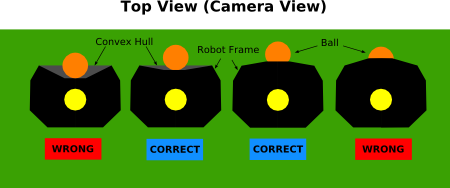
\includegraphics[width=1.0\columnwidth]{img/dribblers_above_view.png}
	\caption{The 80/20 ball covering/holding rule}
	\label{fig:20-rule}
\end{figure}

\item
A robot begins dribbling when it makes contact with the ball and stops dribbling when there is an observable separation between the ball and the robot.

The restriction on dribbling distance was added to prevent a robot with a mechanically superior dribbler having unchallenged control of the ball.
The distance restriction still allows dribblers to be used to aim and receive passes, turn around with the ball, and stop with the ball.
Dribblers can still be used to dribble large distances with the ball as long as the robot periodically loses possession, such as kicking the ball ahead of it as human soccer players often do.
The technical committee expects the distance rule to be self-enforced, i.e., teams will ensure their software complies beforehand and may be asked to demonstrate this prior to a competition.
Referees, though, will still call fouls for violations and may give a caution (yellow card) for situations of repeated violations.

\item
The limitation to kicking speed was added to prevent a robot with a mechanically superior kicker from having too great of an advantage over opponents, or kicking the ball at speed unsafe for spectators.
It is also believed that this will help encourage team play over single robot ability, in a similar way to the restrictions on dribbling.

\item
The current rule about scoring after chip kicks is defined in this section (subsection Indirect Free Kicks) only.
During past competitions, some confusions occurred after robots chipped the ball and thereby caused own goals.
For this reason, a strict interpretation of this rule is provided here:
\begin{itemize}
\item If a robot chips the ball (no matter at which height it travels) at a team mate and the ball subsequently enters the own goal, the opponent team scores.
\item If a robot chips the ball at an opponent and the ball subsequently enters the own goal while staying below 150mm all the time after touching the opponent robot, the opponent team also scores.
\item If a robot chips the ball at an opponent and the ball subsequently enters the own goal after having been above 150mm for some time (and not being in constant touch with the ground afterwards) after touching the opponent robot, the opponent team does not score.
\end{itemize}

\item
The offence on deliberately entering the referee walking area was added to discourage teams from driving through this area to gain tactical advantages.
It is understood that on occasion a robot can enter the area if it is out of control or if it has been pushed into this area.
Such cases should not be considered offences.
However, the final decision as to what constitutes a deliberate violation is left to the referee.

\item
If a tipped over or broken robot does not constitute danger to other robots or humans, neither gives its team unfair advantage, the referee shall allow the game to continue until another game stoppage condition occurs.
The final decision as to what constitutes danger or unfair advantage is left to the referee.

\item
The robot speed limit described in \autoref{subsec:fouls-and-misconduct-disciplinary-sanctions} applies only to cases where the Referee Box is reporting the STOP command during normal play or a penalty shootout.
The intention of this rule is to avoid collisions caused by large numbers of robots moving long distances and to avoid robots accidentally interfering with the referee controlling the ball.
\end{enumerate}
